\documentclass[8pt]{article}

\usepackage{tikz}

\begin{document}
    % blockchain figure
    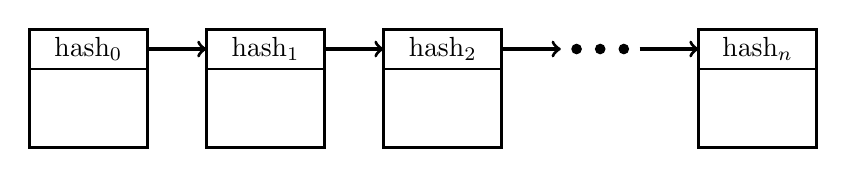
\begin{tikzpicture}
        % boxes (w,l) = (1.5,1.5)
        \draw [very thick] (0,0) rectangle (1.5,1.5);
        \draw [thick] (0,1) -- (1.5,1);
        \node at (0.75,1.25) {hash$_0$};

        \draw [very thick] (2.25,0) rectangle (3.75,1.5);
        \draw [thick] (2.25,1) -- (3.75,1);
        \node at (3,1.25) {hash$_1$};

        \draw [very thick] (4.5,0) rectangle (6,1.5);
        \draw [thick] (4.5,1) -- (6,1);
        \node at (5.25,1.25) {hash$_2$};

        \draw [very thick] (8.5,0) rectangle (10,1.5);
        \draw [thick] (8.5,1) -- (10,1);
        \node at (9.25,1.25) {hash$_n$};

        % lines (length 0.75)
        \draw [->, very thick] (1.5,1.25) -- (2.25,1.25);
        \draw [->, very thick] (3.75,1.25) -- (4.5,1.25);
        \draw [->, very thick] (6,1.25) -- (6.75,1.25);
        \draw [->, very thick] (7.75,1.25) -- (8.5,1.25);

        % dots
        \draw [fill=black] (6.95,1.25) circle (0.06);
        \draw [fill=black] (7.25,1.25) circle (0.06);
        \draw [fill=black] (7.55,1.25) circle (0.06);
    \end{tikzpicture}

    \newpage
    % distributed computing figure
    \begin{center}
    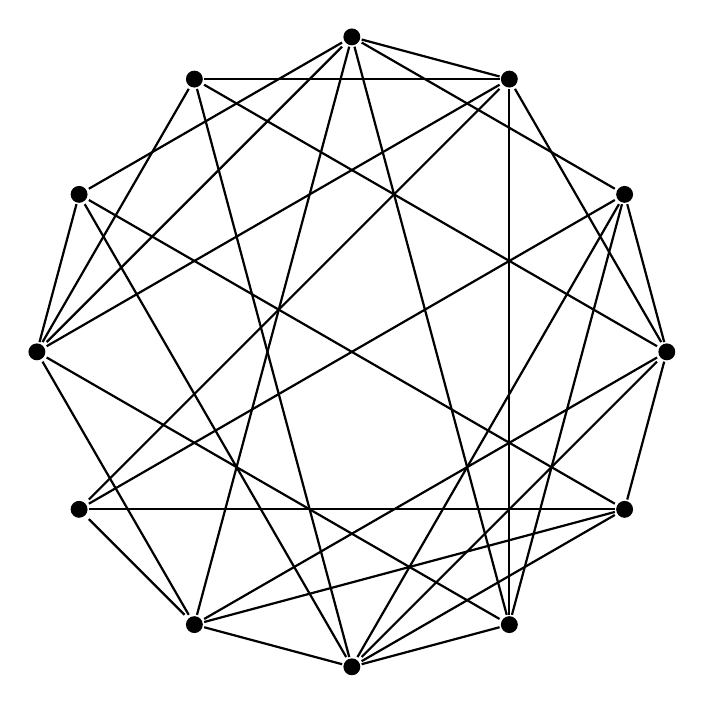
\begin{tikzpicture}
        % dots
        \draw [fill=black] (0,4)       circle (0.1);
        \draw [fill=black] (2,3.464)   circle (0.1);
        \draw [fill=black] (3.464,2)   circle (0.1);
        \draw [fill=black] (4,0)       circle (0.1);
        \draw [fill=black] (3.464,-2)  circle (0.1);
        \draw [fill=black] (2,-3.464)  circle (0.1);
        \draw [fill=black] (0,-4)      circle (0.1);
        \draw [fill=black] (-2,-3.464) circle (0.1);
        \draw [fill=black] (-3.464,-2) circle (0.1);
        \draw [fill=black] (-4,0)      circle (0.1);
        \draw [fill=black] (-3.464,2)  circle (0.1);
        \draw [fill=black] (-2,3.464)  circle (0.1);

        % nodes
        \node (1)         at (0,4) {};
        \node (2)         at (2,3.464) {};
        \node (3)         at (3.464,2)   {};
        \node (4)         at (4,0)       {};
        \node (5)         at (3.464,-2)  {};
        \node (6)         at (2,-3.464)  {};
        \node (7)         at (0,-4)      {};
        \node (8)         at (-2,-3.464) {};
        \node (9)         at (-3.464,-2) {};
        \node (10)        at (-4,0)      {};
        \node (11)        at (-3.464,2)  {};
        \node (12)        at (-2,3.464)  {};

        % lines
        \draw [thick] (1) -- (2);
        \draw [thick] (1) -- (8);
        \draw [thick] (1) -- (11);
        \draw [thick] (1) -- (6);

        \draw [thick] (2) -- (4);
        \draw [thick] (2) -- (10);
        \draw [thick] (2) -- (9);
        \draw [thick] (2) -- (6);

        \draw [thick] (3) -- (1);
        \draw [thick] (3) -- (4);
        \draw [thick] (3) -- (7);
        \draw [thick] (3) -- (6);

        \draw [thick] (4) -- (7);
        \draw [thick] (4) -- (12);
        \draw [thick] (4) -- (8);
        \draw [thick] (4) -- (5);

        \draw [thick] (5) -- (11);
        \draw [thick] (5) -- (7);
        \draw [thick] (5) -- (8);
        \draw [thick] (5) -- (9);

        \draw [thick] (6) -- (10);
        \draw [thick] (6) -- (7);

        \draw [thick] (7) -- (11);
        \draw [thick] (7) -- (12);

        \draw [thick] (8) -- (9);
        \draw [thick] (8) -- (10);
        \draw [thick] (8) -- (7);

        \draw [thick] (9) -- (3);

        \draw [thick] (10) -- (11);
        \draw [thick] (10) -- (1);

        \draw [thick] (12) -- (2);
        \draw [thick] (12) -- (10);
    \end{tikzpicture}
    \end{center}
\end{document}
